\documentclass[12pt, twoside]{article}
\input{../preamble}
\usepackage{pgfplots}
\pgfplotsset{compat=1.18}

\fancyhead[LE]{\thepage}
\fancyhead[RO]{Name: \hspace{4cm} \,\\ \hspace{2.9cm} \,}
\fancyhead[LO]{La Scuola d'Italia / Dr.\ Huson / IB Math \\* 30 March 2026}

\begin{document}
\subsubsection*{6.4 Classwork: Systems of Equations}

\begin{enumerate}[itemsep=0.2cm]

%--- Problem 1: Linear system [7 marks] ---
\item The diagram below shows two lines, $y = 2x - 1$ and $y = -x + 5$.

\begin{center}
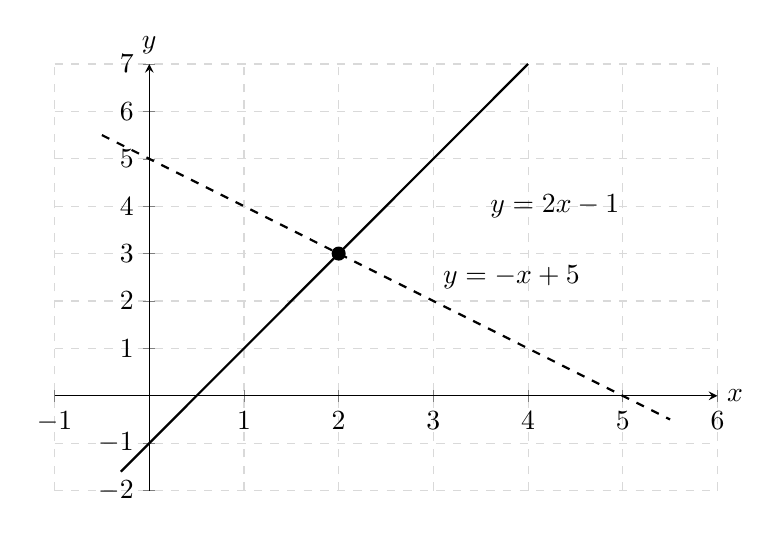
\begin{tikzpicture}
\begin{axis}[
  axis lines=middle,
  xlabel={$x$},
  ylabel={$y$},
  grid=both,
  grid style={dashed, gray!30},
  xmin=-1, xmax=6,
  ymin=-2, ymax=7,
  xtick={-1,0,...,6},
  ytick={-2,-1,...,7},
  width=10cm,
  height=7cm,
  every axis x label/.style={at={(ticklabel* cs:1.0)}, anchor=west},
  every axis y label/.style={at={(ticklabel* cs:1.0)}, anchor=south},
]
  % Line 1: y = 2x - 1
  \addplot[thick, domain=-0.3:4] {2*x - 1};
  % Line 2: y = -x + 5
  \addplot[thick, dashed, domain=-0.5:5.5] {-x + 5};
  % Intersection point
  \node[circle, fill, inner sep=1.8pt] at (axis cs:2,3) {};
  % Labels
  \node[anchor=west] at (axis cs:3.5,4) {$y = 2x - 1$};
  \node[anchor=west] at (axis cs:3,2.5) {$y = -x + 5$};
\end{axis}
\end{tikzpicture}
\end{center}

\begin{enumerate}[itemsep=0.15cm]
  \item Write down the gradient of each line. \hfill [2]
  \item Find the coordinates of the point of intersection by solving
        the system algebraically. \hfill [3]
  \item Verify that the point satisfies both equations. \hfill [2]
\end{enumerate}

\begin{tikzpicture}
  \draw (0,0) rectangle (15.5,7);
  \foreach \y in {1,2,...,6} \draw [dotted] (0.5,\y)--(15,\y);
\end{tikzpicture}

\newpage

%--- Problem 2: Quadratic system [8 marks] ---
\item The diagram below shows two parabolas, $y = x^2 - 4x + 3$ and
$y = -x^2 + 2x + 3$.

\begin{center}
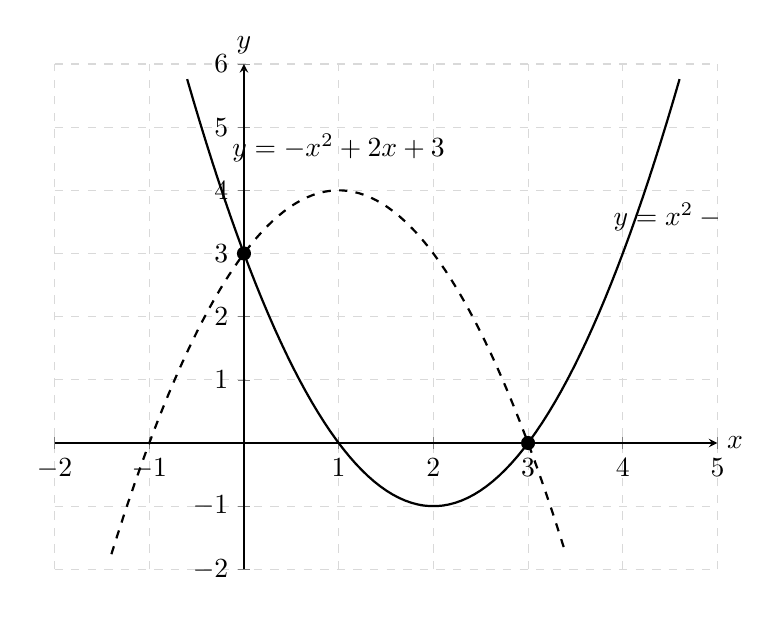
\begin{tikzpicture}
\begin{axis}[
  axis lines=middle,
  xlabel={$x$},
  ylabel={$y$},
  grid=both,
  grid style={dashed, gray!30},
  xmin=-2, xmax=5,
  ymin=-2, ymax=6,
  xtick={-2,-1,...,5},
  ytick={-2,-1,...,6},
  width=10cm,
  height=8cm,
  every axis x label/.style={at={(ticklabel* cs:1.0)}, anchor=west},
  every axis y label/.style={at={(ticklabel* cs:1.0)}, anchor=south},
]
  % Parabola 1: y = x^2 - 4x + 3 (opens up, vertex at (2,-1))
  \addplot[thick, domain=-0.6:4.6, samples=80] {x^2 - 4*x + 3};
  % Parabola 2: y = -x^2 + 2x + 3 (opens down, vertex at (1,4))
  \addplot[thick, dashed, domain=-1.4:3.4, samples=80] {-x^2 + 2*x + 3};
  % Intersection points
  \node[circle, fill, inner sep=1.8pt] at (axis cs:0,3) {};
  \node[circle, fill, inner sep=1.8pt] at (axis cs:3,0) {};
  % Labels
  \node[anchor=south west] at (axis cs:3.8,3.2) {$y = x^2 - 4x + 3$};
  \node[anchor=south] at (axis cs:1,4.3) {$y = -x^2 + 2x + 3$};
\end{axis}
\end{tikzpicture}
\end{center}

\begin{enumerate}[itemsep=0.15cm]
  \item Show that the $x$-coordinates of the points of intersection
        satisfy $2x^2 - 6x = 0$. \hfill [2]
  \item Hence find the $x$-coordinates of the points of intersection. \hfill [2]
  \item Find the coordinates of both points of intersection. \hfill [2]
  \item Find the coordinates of the vertex of $y = x^2 - 4x + 3$. \hfill [2]
\end{enumerate}

\begin{tikzpicture}
  \draw (0,0) rectangle (15.5,5);
  \foreach \y in {1,2,...,4} \draw [dotted] (0.5,\y)--(15,\y);
\end{tikzpicture}

\end{enumerate}
\end{document}

Solutions
  Problem 1 — Linear system:
  - (a) Gradient of y = 2x - 1: m = 2. Gradient of y = -x + 5: m = -1
  - (b) 2x - 1 = -x + 5 -> 3x = 6 -> x = 2. y = 2(2) - 1 = 3. Point: (2, 3)
  - (c) Check: y = 2(2) - 1 = 3. y = -(2) + 5 = 3. Both true.

  Problem 2 — Quadratic system:
  - (a) x^2 - 4x + 3 = -x^2 + 2x + 3 -> 2x^2 - 6x = 0
  - (b) 2x(x - 3) = 0 -> x = 0 or x = 3
  - (c) x = 0: y = 3 -> (0, 3). x = 3: y = 9 - 12 + 3 = 0 -> (3, 0)
  - (d) x = 4/2 = 2. y = 4 - 8 + 3 = -1. Vertex = (2, -1)
